\documentclass[a4paper,12pt]{article}
\usepackage{tikz}
\usetikzlibrary{arrows,shapes}

\usepackage[english]{babel}
\usepackage{courier}


\usepackage[T1]{fontenc}

\usepackage[pdftex, colorlinks=true]{hyperref}

\usepackage{listings}
\lstloadlanguages{python}
\lstset{language=python,numbers=left,numberstyle=\tiny,emph={self},emphstyle=\color{blue},basicstyle=\footnotesize}
\title{How To Become a Production Manager}
\author{S.~Poss}

\begin{document}
\tikzstyle{decision} = [diamond, draw, text badly centered, node distance=2.8cm]
\tikzstyle{block} = [rectangle, draw, text centered, rounded corners, node distance=2.2cm]
\tikzstyle{autoblock} = [rectangle, draw, text centered, rounded corners, node distance=2.2cm]
\tikzstyle{line} = [draw, -triangle 90]
\tikzstyle{dline} = [draw, dashed, -triangle 90]

\maketitle
\abstract{This document presents the method for group production managers to
extend existing productions.}

\tableofcontents

\section{Introduction}
There are at least seven different analysis being performed in parallel. There
are as many people looking at the corresponding samples. It would be more
convenient if every analysis gets a responsible for the production. Its task is
only to extend the existing productions, not to submit new ones. 

Submission will
still be done by a very restricted set of people to ensure harmony of
production definitions. 

The defined production managers should have the right to extend, stop and
restart existing productions. This can fortunately be done  via the web
interface. The interactions with the production system will be detailed in the
following section, and the limitations that should be respected and eventually
enforced will be detailed in the last section.

\section{Interacting with the production system}
To interact with the system, you should first be connected with your browser
to\\
\url{https://ilcdirac.cern.ch/DIRAC/ILC-Production/ilc\_user/jobs/ProductionMonitor/display}

You should have something like the Fig.~\ref{fig:welcome} as a screen. If not refer to
section~\ref{sec:problem}.
\begin{figure}[h]
\begin{center}
\begin{tikzpicture}[scale=0.8,auto]
\node{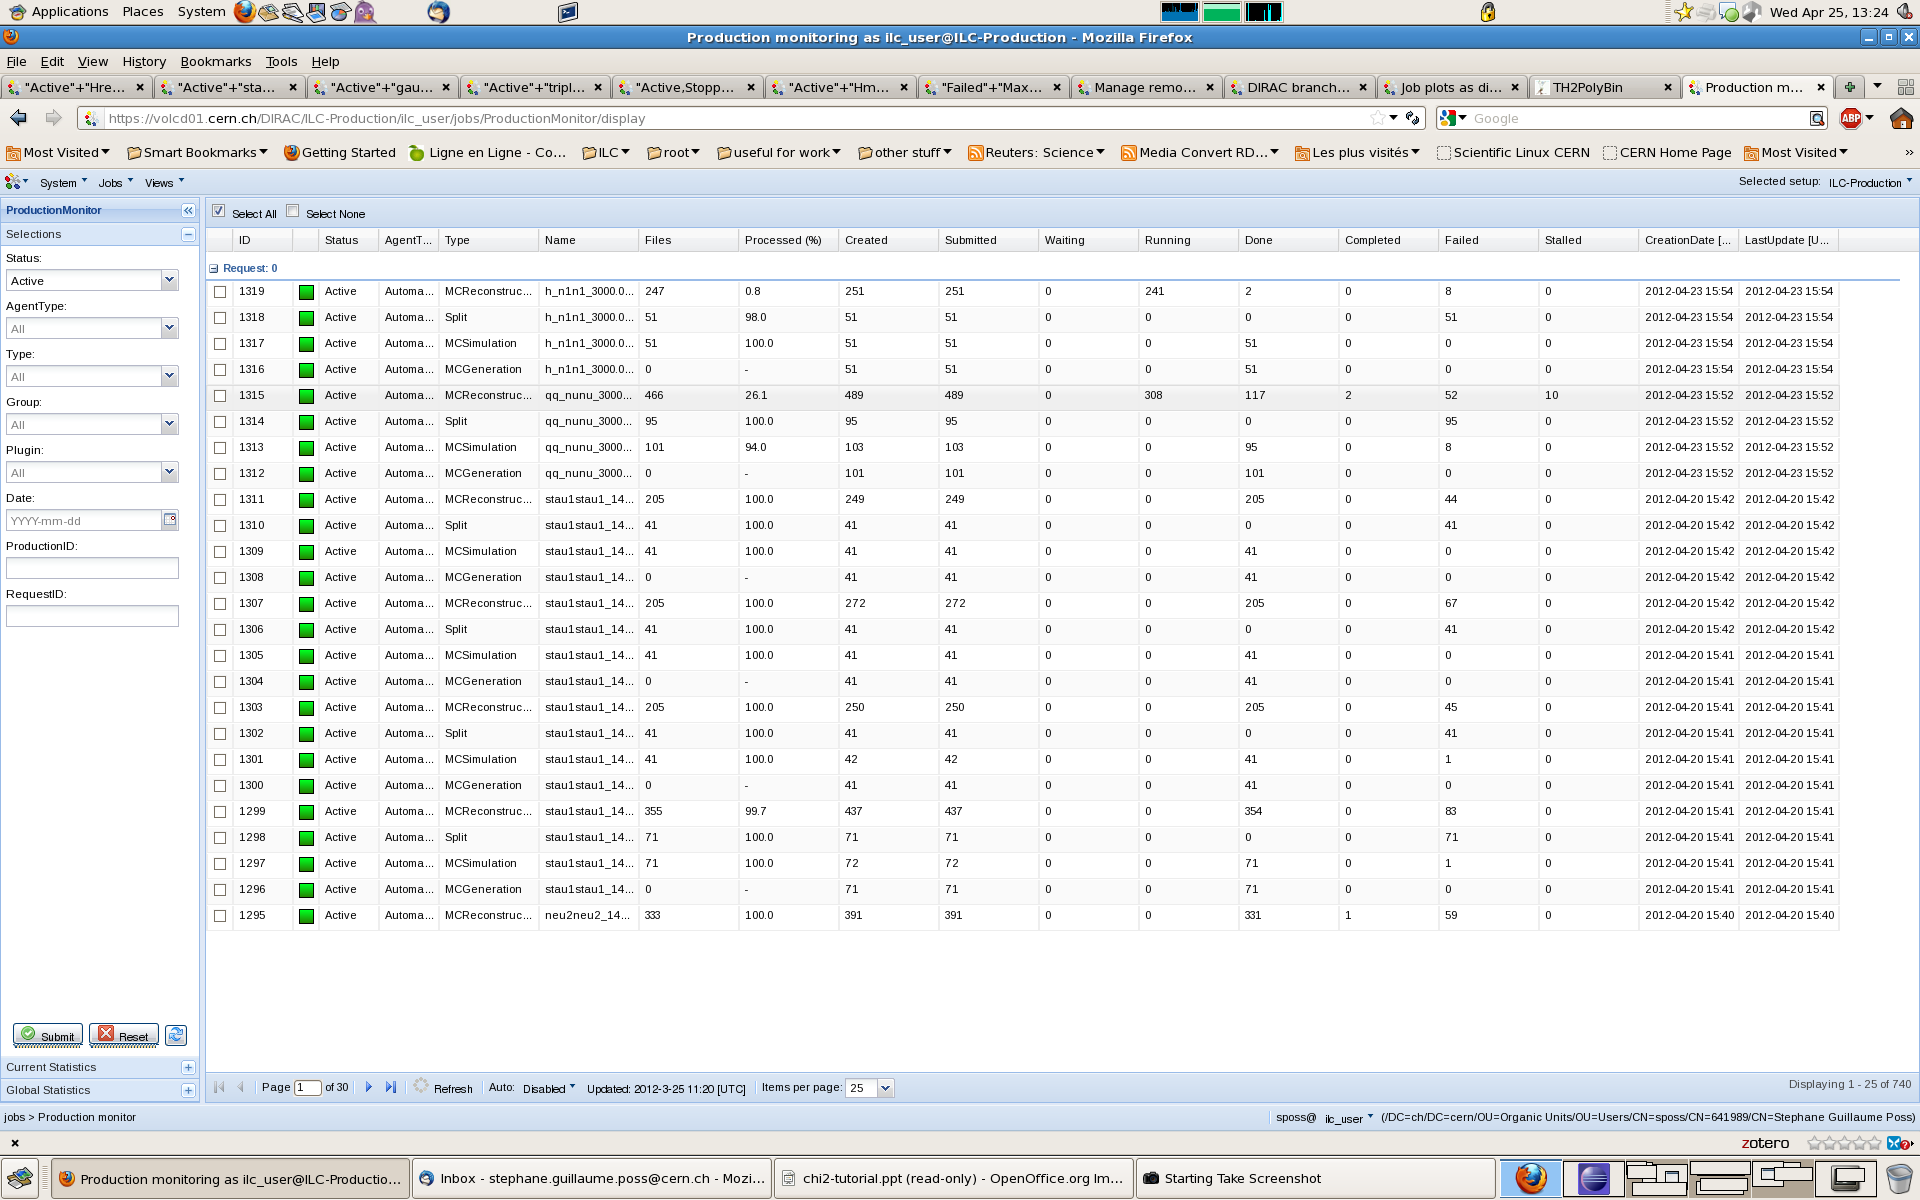
\includegraphics[width=14cm]{welcomescreen.png}};
\end{tikzpicture}
\end{center}
\caption{Welcome screen of the production manager page.}\label{fig:welcome}
\end{figure}

What you need to do is to change the group in which you are, as most
interactions are restricted. For this you need to look at the little button
indicated in Fig.~\ref{fig:welcome2}. 
\begin{figure}[h]
\begin{center}
\begin{tikzpicture}
\node {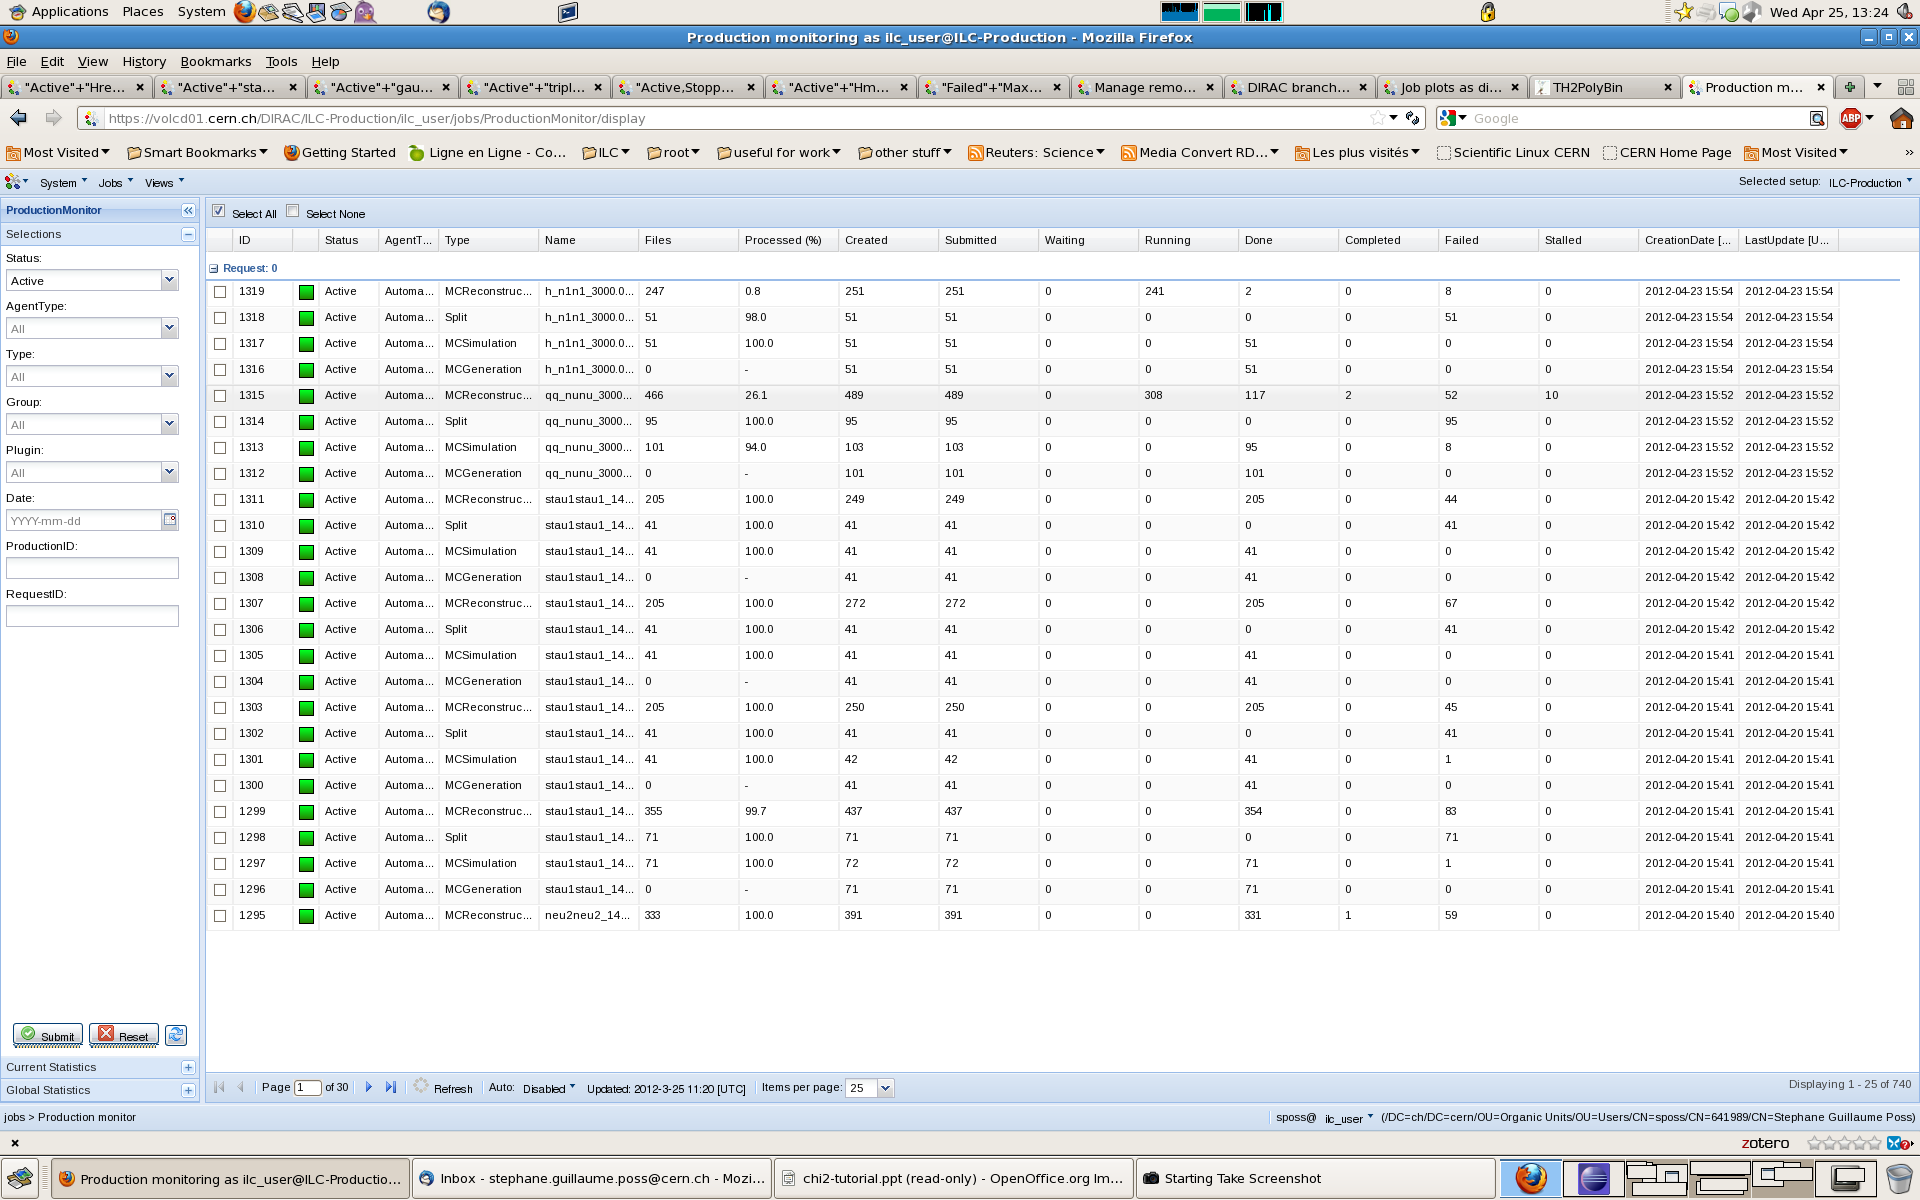
\includegraphics[width=14cm]{welcomescreen.png}};
\draw [->,color=red] (3.4,-2.1) -- (3.,-3.7);
\end{tikzpicture}
\end{center}
\caption{Click here.}\label{fig:welcome2}
\end{figure}
There you will click and select {\color{red} ilc\_prodman}.

And you should have something like what is shown in Fig.~\ref{fig:welcome3}.
\begin{figure}[h]
\begin{center}
\begin{tikzpicture}[scale=0.8,auto]
\node{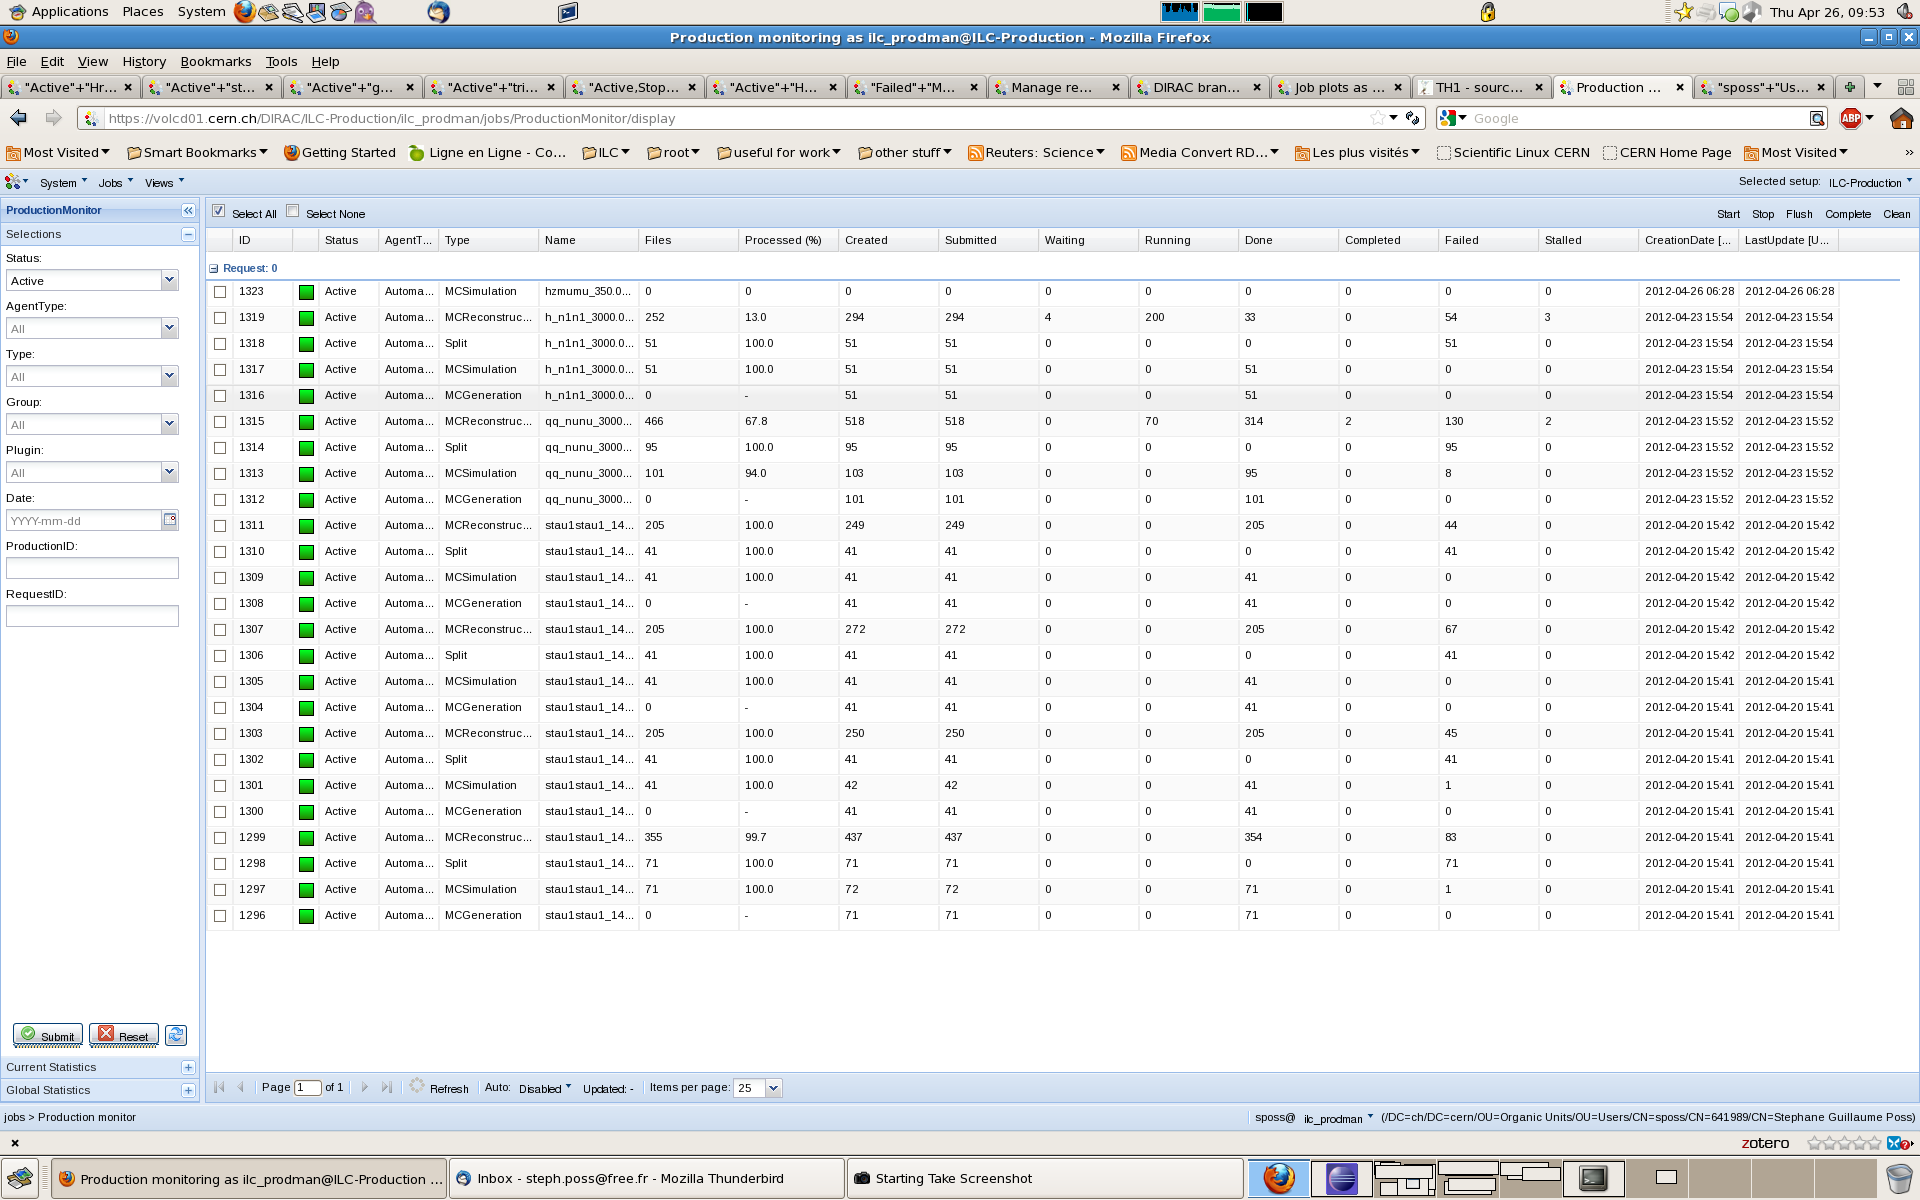
\includegraphics[width=14cm]{welcomescreen2.png}};
\end{tikzpicture}
\end{center}
\caption{This is what you should end up with.}\label{fig:welcome3}
\end{figure}
From there, you should select the productions you want, using the fields on the
left. In those fields, you should select in particular the \emph{Type} field,
and the value {\color{red}MCGeneration} that is the type that can be extended.

You should also check the status of the other productions (Type and Group), so
that you get an idea of the current activities.

Check the production properties by right-clicking one, and on \emph{Additional
Params}. There you'll see all the production properties, in particular, you
need to check the \emph{nbevts} field that tells you how many events there are in
each job running and to come.

Once you have selected the productions you want to extend, just left-click on
one, go to \emph{Actions} then \emph{extend}. There you have a box asking for a
number. This number is the number of jobs you want to add.

Click \emph{OK} and the page should reload with small changes: the numbers in
each column is updated and a little indicator gives the delta. 

In case of rapid increase of the \emph{Failed} column content, you can check the
jobs themselves, but not obtain the sandboxes (only the ilc\_prod group can).
Nevertheless, from the job monitoring, the ApplicationStatus usually gives the
reason of the failures. 

In any case, the administrators should be warned. The affected productions
should be stopped. For that, click on the box on the left for every production
in question, then on the top right, click \emph{stop}.

\section{Meaning of the other actions}
We saw \emph{Extend} and \emph{Stop}, but there are other possibilities:
\begin{itemize}
  \item[Start] Start a production: useful when a production was stopped.
  \item[Flush] Not really useful for us: when input files are grouped together,
  this allows to create productions with the remaining files. This is necessary
  when you group the files by 10 and you have a total of 106 files. The last job
  created with \emph{Flush} will have only 6 files in. 
  \item[Complete] Make the production finished: remove all jobs, clean the
  production system. Can also mark the log files as archive, but we don't have
  anything to treat them. Then the productions cannot be resurrected. Please
  leave that for central admins.
  \item[Clean] A bit like the Complete above, but also removes any file
  produced. Also avoid using this.
\end{itemize}

\section{Limitations}
When you need a lot of events (or Jobs), you need to make sure you do not
interfere with others' activities. For that, make sure you have checked how many
jobs in total are waiting. The jobs are submitted by 50, whatever the value you
put in, but if there is nothing running, if you put a very large value, you
might end up with many of your jobs waiting when others arrive, therefore
blocking other users. I suggest to only submit by chunks of 200 per day and per
production max. 

As a system/production manager, I will monitor the evolution of the system, and
I will enforce some fair share. If someone does not play well with others, he
might loose his privileges.

\section{What if it does not work?}\label{sec:problem}
Well, too bad.\footnote{You are allowed to contact me for assitance.}
\end{document}